
%% bare_jrnl_transmag.tex
%% V1.4b
%% 2015/08/26
%% by Michael Shell
%% see http://www.michaelshell.org/
%% for current contact information.
%%
%% This is a skeleton file demonstrating the use of IEEEtran.cls
%% (requires IEEEtran.cls version 1.8b or later) with an IEEE 
%% Transactions on Magnetics journal paper.
%%
%% Support sites:
%% http://www.michaelshell.org/tex/ieeetran/
%% http://www.ctan.org/pkg/ieeetran
%% and
%% http://www.ieee.org/

%%*************************************************************************
%% Legal Notice:
%% This code is offered as-is without any warranty either expressed or
%% implied; without even the implied warranty of MERCHANTABILITY or
%% FITNESS FOR A PARTICULAR PURPOSE! 
%% User assumes all risk.
%% In no event shall the IEEE or any contributor to this code be liable for
%% any damages or losses, including, but not limited to, incidental,
%% consequential, or any other damages, resulting from the use or misuse
%% of any information contained here.
%%
%% All comments are the opinions of their respective authors and are not
%% necessarily endorsed by the IEEE.
%%
%% This work is distributed under the LaTeX Project Public License (LPPL)
%% ( http://www.latex-project.org/ ) version 1.3, and may be freely used,
%% distributed and modified. A copy of the LPPL, version 1.3, is included
%% in the base LaTeX documentation of all distributions of LaTeX released
%% 2003/12/01 or later.
%% Retain all contribution notices and credits.
%% ** Modified files should be clearly indicated as such, including  **
%% ** renaming them and changing author support contact information. **
%%*************************************************************************


% *** Authors should verify (and, if needed, correct) their LaTeX system  ***
% *** with the testflow diagnostic prior to trusting their LaTeX platform ***
% *** with production work. The IEEE's font choices and paper sizes can   ***
% *** trigger bugs that do not appear when using other class files.       ***                          ***
% The testflow support page is at:
% http://www.michaelshell.org/tex/testflow/



\documentclass[journal,transmag]{IEEEtran}
%\usepackage[style=authoryear,backend=bibtex]{biblatex} %backend tells biblatex what you will be using to process the bibliography file
%\addbibresource{refer.bib}
\usepackage{graphicx}
\usepackage{url}
%
% If IEEEtran.cls has not been installed into the LaTeX system files,
% manually specify the path to it like:
% \documentclass[journal]{../sty/IEEEtran}





% Some very useful LaTeX packages include:
% (uncomment the ones you want to load)


% *** MISC UTILITY PACKAGES ***
%
%\usepackage{ifpdf}
% Heiko Oberdiek's ifpdf.sty is very useful if you need conditional
% compilation based on whether the output is pdf or dvi.
% usage:
% \ifpdf
%   % pdf code
% \else
%   % dvi code
% \fi
% The latest version of ifpdf.sty can be obtained from:
% http://www.ctan.org/pkg/ifpdf
% Also, note that IEEEtran.cls V1.7 and later provides a builtin
% \ifCLASSINFOpdf conditional that works the same way.
% When switching from latex to pdflatex and vice-versa, the compiler may
% have to be run twice to clear warning/error messages.






% *** CITATION PACKAGES ***
%
\usepackage{cite}
\usepackage{array}
% cite.sty was written by Donald Arseneau
% V1.6 and later of IEEEtran pre-defines the format of the cite.sty package
% \cite{} output to follow that of the IEEE. Loading the cite package will
% result in citation numbers being automatically sorted and properly
% "compressed/ranged". e.g., [1], [9], [2], [7], [5], [6] without using
% cite.sty will become [1], [2], [5]--[7], [9] using cite.sty. cite.sty's
% \cite will automatically add leading space, if needed. Use cite.sty's
% noadjust option (cite.sty V3.8 and later) if you want to turn this off
% such as if a citation ever needs to be enclosed in parenthesis.
% cite.sty is already installed on most LaTeX systems. Be sure and use
% version 5.0 (2009-03-20) and later if using hyperref.sty.
% The latest version can be obtained at:
% http://www.ctan.org/pkg/cite
% The documentation is contained in the cite.sty file itself.






% *** GRAPHICS RELATED PACKAGES ***
%
\ifCLASSINFOpdf
  % \usepackage[pdftex]{graphicx}
  % declare the path(s) where your graphic files are
  % \graphicspath{{../pdf/}{../jpeg/}}
  % and their extensions so you won't have to specify these with
  % every instance of \includegraphics
  % \DeclareGraphicsExtensions{.pdf,.jpeg,.png}
\else
  % or other class option (dvipsone, dvipdf, if not using dvips). graphicx
  % will default to the driver specified in the system graphics.cfg if no
  % driver is specified.
  % \usepackage[dvips]{graphicx}
  % declare the path(s) where your graphic files are
  % \graphicspath{{../eps/}}
  % and their extensions so you won't have to specify these with
  % every instance of \includegraphics
  % \DeclareGraphicsExtensions{.eps}
\fi
% graphicx was written by David Carlisle and Sebastian Rahtz. It is
% required if you want graphics, photos, etc. graphicx.sty is already
% installed on most LaTeX systems. The latest version and documentation
% can be obtained at: 
% http://www.ctan.org/pkg/graphicx
% Another good source of documentation is "Using Imported Graphics in
% LaTeX2e" by Keith Reckdahl which can be found at:
% http://www.ctan.org/pkg/epslatex
%
% latex, and pdflatex in dvi mode, support graphics in encapsulated
% postscript (.eps) format. pdflatex in pdf mode supports graphics
% in .pdf, .jpeg, .png and .mps (metapost) formats. Users should ensure
% that all non-photo figures use a vector format (.eps, .pdf, .mps) and
% not a bitmapped formats (.jpeg, .png). The IEEE frowns on bitmapped formats
% which can result in "jaggedy"/blurry rendering of lines and letters as
% well as large increases in file sizes.
%
% You can find documentation about the pdfTeX application at:
% http://www.tug.org/applications/pdftex




% *** MATH PACKAGES ***
%
%\usepackage{amsmath}
% A popular package from the American Mathematical Society that provides
% many useful and powerful commands for dealing with mathematics.
%
% Note that the amsmath package sets \interdisplaylinepenalty to 10000
% thus preventing page breaks from occurring within multiline equations. Use:
%\interdisplaylinepenalty=2500
% after loading amsmath to restore such page breaks as IEEEtran.cls normally
% does. amsmath.sty is already installed on most LaTeX systems. The latest
% version and documentation can be obtained at:
% http://www.ctan.org/pkg/amsmath





% *** SPECIALIZED LIST PACKAGES ***
%
%\usepackage{algorithmic}
% algorithmic.sty was written by Peter Williams and Rogerio Brito.
% This package provides an algorithmic environment fo describing algorithms.
% You can use the algorithmic environment in-text or within a figure
% environment to provide for a floating algorithm. Do NOT use the algorithm
% floating environment provided by algorithm.sty (by the same authors) or
% algorithm2e.sty (by Christophe Fiorio) as the IEEE does not use dedicated
% algorithm float types and packages that provide these will not provide
% correct IEEE style captions. The latest version and documentation of
% algorithmic.sty can be obtained at:
% http://www.ctan.org/pkg/algorithms
% Also of interest may be the (relatively newer and more customizable)
% algorithmicx.sty package by Szasz Janos:
% http://www.ctan.org/pkg/algorithmicx




% *** ALIGNMENT PACKAGES ***
%
%\usepackage{array}
% Frank Mittelbach's and David Carlisle's array.sty patches and improves
% the standard LaTeX2e array and tabular environments to provide better
% appearance and additional user controls. As the default LaTeX2e table
% generation code is lacking to the point of almost being broken with
% respect to the quality of the end results, all users are strongly
% advised to use an enhanced (at the very least that provided by array.sty)
% set of table tools. array.sty is already installed on most systems. The
% latest version and documentation can be obtained at:
% http://www.ctan.org/pkg/array


% IEEEtran contains the IEEEeqnarray family of commands that can be used to
% generate multiline equations as well as matrices, tables, etc., of high
% quality.




% *** SUBFIGURE PACKAGES ***
%\ifCLASSOPTIONcompsoc
%  \usepackage[caption=false,font=normalsize,labelfont=sf,textfont=sf]{subfig}
%\else
%  \usepackage[caption=false,font=footnotesize]{subfig}
%\fi
% subfig.sty, written by Steven Douglas Cochran, is the modern replacement
% for subfigure.sty, the latter of which is no longer maintained and is
% incompatible with some LaTeX packages including fixltx2e. However,
% subfig.sty requires and automatically loads Axel Sommerfeldt's caption.sty
% which will override IEEEtran.cls' handling of captions and this will result
% in non-IEEE style figure/table captions. To prevent this problem, be sure
% and invoke subfig.sty's "caption=false" package option (available since
% subfig.sty version 1.3, 2005/06/28) as this is will preserve IEEEtran.cls
% handling of captions.
% Note that the Computer Society format requires a larger sans serif font
% than the serif footnote size font used in traditional IEEE formatting
% and thus the need to invoke different subfig.sty package options depending
% on whether compsoc mode has been enabled.
%
% The latest version and documentation of subfig.sty can be obtained at:
% http://www.ctan.org/pkg/subfig



% *** FLOAT PACKAGES ***
%
%\usepackage{fixltx2e}
% fixltx2e, the successor to the earlier fix2col.sty, was written by
% Frank Mittelbach and David Carlisle. This package corrects a few problems
% in the LaTeX2e kernel, the most notable of which is that in current
% LaTeX2e releases, the ordering of single and double column floats is not
% guaranteed to be preserved. Thus, an unpatched LaTeX2e can allow a
% single column figure to be placed prior to an earlier double column
% figure.
% Be aware that LaTeX2e kernels dated 2015 and later have fixltx2e.sty's
% corrections already built into the system in which case a warning will
% be issued if an attempt is made to load fixltx2e.sty as it is no longer
% needed.
% The latest version and documentation can be found at:
% http://www.ctan.org/pkg/fixltx2e


%\usepackage{stfloats}
% stfloats.sty was written by Sigitas Tolusis. This package gives LaTeX2e
% the ability to do double column floats at the bottom of the page as well
% as the top. (e.g., "\begin{figure*}[!b]" is not normally possible in
% LaTeX2e). It also provides a command:
%\fnbelowfloat
% to enable the placement of footnotes below bottom floats (the standard
% LaTeX2e kernel puts them above bottom floats). This is an invasive package
% which rewrites many portions of the LaTeX2e float routines. It may not work
% with other packages that modify the LaTeX2e float routines. The latest
% version and documentation can be obtained at:
% http://www.ctan.org/pkg/stfloats
% Do not use the stfloats baselinefloat ability as the IEEE does not allow
% \baselineskip to stretch. Authors submitting work to the IEEE should note
% that the IEEE rarely uses double column equations and that authors should try
% to avoid such use. Do not be tempted to use the cuted.sty or midfloat.sty
% packages (also by Sigitas Tolusis) as the IEEE does not format its papers in
% such ways.
% Do not attempt to use stfloats with fixltx2e as they are incompatible.
% Instead, use Morten Hogholm'a dblfloatfix which combines the features
% of both fixltx2e and stfloats:
%
% \usepackage{dblfloatfix}
% The latest version can be found at:
% http://www.ctan.org/pkg/dblfloatfix




%\ifCLASSOPTIONcaptionsoff
%  \usepackage[nomarkers]{endfloat}
% \let\MYoriglatexcaption\caption
% \renewcommand{\caption}[2][\relax]{\MYoriglatexcaption[#2]{#2}}
%\fi
% endfloat.sty was written by James Darrell McCauley, Jeff Goldberg and 
% Axel Sommerfeldt. This package may be useful when used in conjunction with 
% IEEEtran.cls'  captionsoff option. Some IEEE journals/societies require that
% submissions have lists of figures/tables at the end of the paper and that
% figures/tables without any captions are placed on a page by themselves at
% the end of the document. If needed, the draftcls IEEEtran class option or
% \CLASSINPUTbaselinestretch interface can be used to increase the line
% spacing as well. Be sure and use the nomarkers option of endfloat to
% prevent endfloat from "marking" where the figures would have been placed
% in the text. The two hack lines of code above are a slight modification of
% that suggested by in the endfloat docs (section 8.4.1) to ensure that
% the full captions always appear in the list of figures/tables - even if
% the user used the short optional argument of \caption[]{}.
% IEEE papers do not typically make use of \caption[]'s optional argument,
% so this should not be an issue. A similar trick can be used to disable
% captions of packages such as subfig.sty that lack options to turn off
% the subcaptions:
% For subfig.sty:
% \let\MYorigsubfloat\subfloat
% \renewcommand{\subfloat}[2][\relax]{\MYorigsubfloat[]{#2}}
% However, the above trick will not work if both optional arguments of
% the \subfloat command are used. Furthermore, there needs to be a
% description of each subfigure *somewhere* and endfloat does not add
% subfigure captions to its list of figures. Thus, the best approach is to
% avoid the use of subfigure captions (many IEEE journals avoid them anyway)
% and instead reference/explain all the subfigures within the main caption.
% The latest version of endfloat.sty and its documentation can obtained at:
% http://www.ctan.org/pkg/endfloat
%
% The IEEEtran \ifCLASSOPTIONcaptionsoff conditional can also be used
% later in the document, say, to conditionally put the References on a 
% page by themselves.




% *** PDF, URL AND HYPERLINK PACKAGES ***
%
%\usepackage{url}
% url.sty was written by Donald Arseneau. It provides better support for
% handling and breaking URLs. url.sty is already installed on most LaTeX
% systems. The latest version and documentation can be obtained at:
% http://www.ctan.org/pkg/url
% Basically, \url{my_url_here}.




% *** Do not adjust lengths that control margins, column widths, etc. ***
% *** Do not use packages that alter fonts (such as pslatex).         ***
% There should be no need to do such things with IEEEtran.cls V1.6 and later.
% (Unless specifically asked to do so by the journal or conference you plan
% to submit to, of course. )


% correct bad hyphenation here
\hyphenation{op-tical net-works semi-conduc-tor}


\begin{document}
%
% paper title
% Titles are generally capitalized except for words such as a, an, and, as,
% at, but, by, for, in, nor, of, on, or, the, to and up, which are usually
% not capitalized unless they are the first or last word of the title.
% Linebreaks \\ can be used within to get better formatting as desired.
% Do not put math or special symbols in the title.
\title{Indoor Localization system using Time of Flight in UWB spectrum}

% author names and affiliations
% transmag papers use the long conference author name format.

\author{\IEEEauthorblockN{Anirban Ghosh,
Albert Davies,
Tejus Siddagangaiah}
\IEEEauthorblockA{Electrical and Computer Engineering Department,
Carnegie Mellon University, Pittsburgh, PA 15213 USA}}




% The paper headers
%\markboth{Journal of \LaTeX\ Class Files,~Vol.~14, No.~8, August~2015}%
%{Shell \MakeLowercase{\textit{et al.}}: Bare Demo of IEEEtran.cls for IEEE Transactions on Magnetics Journals}
% The only time the second header will appear is for the odd numbered pages
% after the title page when using the twoside option.
% 
% *** Note that you probably will NOT want to include the author's ***
% *** name in the headers of peer review papers.                   ***
% You can use \ifCLASSOPTIONpeerreview for conditional compilation here if
% you desire.




% If you want to put a publisher's ID mark on the page you can do it like
% this:
%\IEEEpubid{0000--0000/00\$00.00~\copyright~2015 IEEE}
% Remember, if you use this you must call \IEEEpubidadjcol in the second
% column for its text to clear the IEEEpubid mark.



% use for special paper notices
%\IEEEspecialpapernotice{(Invited Paper)}


% for Transactions on Magnetics papers, we must declare the abstract and
% index terms PRIOR to the title within the \IEEEtitleabstractindextext
% IEEEtran command as these need to go into the title area created by
% \maketitle.
% As a general rule, do not put math, special symbols or citations
% in the abstract or keywords.
%\IEEEtitleabstractindextext{%


% Note that keywords are not normally used for peerreview papers.
%\begin{IEEEkeywords}
%IEEE, IEEEtran, IEEE Transactions on Magnetics, journal, \LaTeX, %magnetics, paper, template.
%\end{IEEEkeywords}}



% make the title area
\maketitle


% To allow for easy dual compilation without having to reenter the
% abstract/keywords data, the \IEEEtitleabstractindextext text will
% not be used in maketitle, but will appear (i.e., to be "transported")
% here as \IEEEdisplaynontitleabstractindextext when the compsoc 
% or transmag modes are not selected <OR> if conference mode is selected 
% - because all conference papers position the abstract like regular
% papers do.
\IEEEdisplaynontitleabstractindextext
% \IEEEdisplaynontitleabstractindextext has no effect when using
% compsoc or transmag under a non-conference mode.







% For peer review papers, you can put extra information on the cover
% page as needed:
% \ifCLASSOPTIONpeerreview
% \begin{center} \bfseries EDICS Category: 3-BBND \end{center}
% \fi
%
% For peerreview papers, this IEEEtran command inserts a page break and
% creates the second title. It will be ignored for other modes.
\IEEEpeerreviewmaketitle

\begin{abstract}
Positioning systems based on GPS have become ubiquitous over the past few decades. Due to the attenuation of GPS signals, they cannot be used in an indoor setting for localization. In recent years, multiple attempts have been made to design a localization system for indoor applications. Indoor localization has the potential for trans-formative impact in a wide variety of applications like augmented reality, indoor navigation, asset tracking and advertising. Due to the inherent nature of the applications, high accuracy as well as energy efficiency is required.
Based on the target application, various methods and system architectures have been proposed using broadcast-based technologies(RFID\cite{bouet2008rfid}, BLE\cite{alps}, WiFi\cite{yang2012locating}, Ultrasound\cite{ultrasonic}) and motion based algorithms(Inertial based sensing)\cite{li2012reliable}.   

In our work, we develop a system for Indoor Localization to track mobile TAG nodes in an indoor setting with multiple anchor nodes whose coordinates are known. We use Decawave's DWM1000 modules to perform accurate ranging and Arduino UNO WiFi modules to control the modules and perform basic computation. We achieve a best case and average accuracy of 10cm and 20 cm respectively across each axes.
\footnote{Git Repository: \href{https://github.com/tejus26/Indoor-Localization.git}}
\end{abstract}

\section{Introduction}

\cite{bouet2008rfid} surveys various RFID based localization strategies. RFID based localization schemes suffer from need for several active RFID anchors to be able to localize accurately. WiFi based localization schemes require intensive calibration in the area of localization. Several methods have been proposed to crowd-source the RSSI values from different WiFi access points \cite{yang2012locating}. Another approach to this problem has been to use two different mediums and measure the time difference of arrival of signals in both the mediums. This is the approach used by \cite{alps} wherein the different speed of travel of bluetooth and ultrasonic waves are used to estimate distance. Inertial based localization strategies \cite{li2012reliable} fail to achieve sub metre accuracy due to drift from initial calibration that compounds with time. A recent development in the indoor localization domain has been the success of UWB based methods\cite{uwb}. The promise of UWB based localization was witnessed when DWM1000, a UWB localization chip won the Microsoft indoor localization competition in the year 2015. Some of the current commercial positioning systems include the Ubisense technology, Time Domain technology, Decawave technology, Zebra technology, Nanotron technology and Apple's iBeacon. The advantages and disadvantages of these systems are investigated in \cite{yavari2014ultra}

\section{Architecture}
This section describes the overall system architecture as well as some of the design decisions we took during the course of this project.  We begin by describing the different localization algorithms.  Next, we describe the software architecture and finally describe the hardware design choices.   
\subsection{Localization Algorithm}
There are two predominant methods used in the field of localization (both indoor and outdoor).  The first is time-of-flight measurement. This computes the point-to-point distance between two nodes based on the round trip time of a time-stamped packet travelling in a known medium. Alternatively, time-difference-of-arrival uses the difference in time of arrival between multiple packets sent from the Tag to time-synchronized anchor nodes. These schemes and their corresponding equations are explained in \cite{gaffney2008considerations}

\subsubsection{Time of Flight}
As shown in Figure \ref{fig:tof}, the time-of-flight (TOF) method computes the distance between the two nodes by measuring the round-trip time of a time stamped packet.  As given by equations \ref{eq:tof} and \ref{eq:distcalc} node 1 sends the packet (t1 at t1\textsubscript{tx})  and waits for node 2 to respond (t2 at t2\textsubscript{rx}).  Upon receiving the packet, node 2 responds with another packet, which contains the time difference between when node 2 receives the first packet and sends the response.  When node 1 receives node 2's response, it calculates the difference between when it sent the first packet and when it receives the response.  Node 2's response latency, which is embedded in the response packet is then subtracted from this time to obtain the true round trip time.  The packet travels twice the distance between the nodes, so the distance between the two nodes is equal to half the round trip time multiplied by the speed of the packet in the given medium, as given by \ref{eq:distcalc}.  In case of the DWM1000, the speed of the packet is the speed of light in air and in case of ultrasonic methods, this is the speed of sound in air and so on.  In 3D space, the distance computed between an anchor and a tag defines a sphere where the tag must lie.  The tag must then periodically find its distance from four different anchor nodes placed around the room.  The 3D location of the tag will then be the intersection of the four spherical surfaces generated in this process.  The advantage of the TOF method is that it is much simpler to implement well and does not require time synchronization between the nodes. However, since the round trip time is measured, this method requires the delay added due to transducers (RF circuits in our case) and the response time of node 2 to be modelled accurately.  In the case of the DWM1000 modules, these parameters are factory calibrated and don't cause any accuracy issues.  


\begin{figure}[!h]
\centering
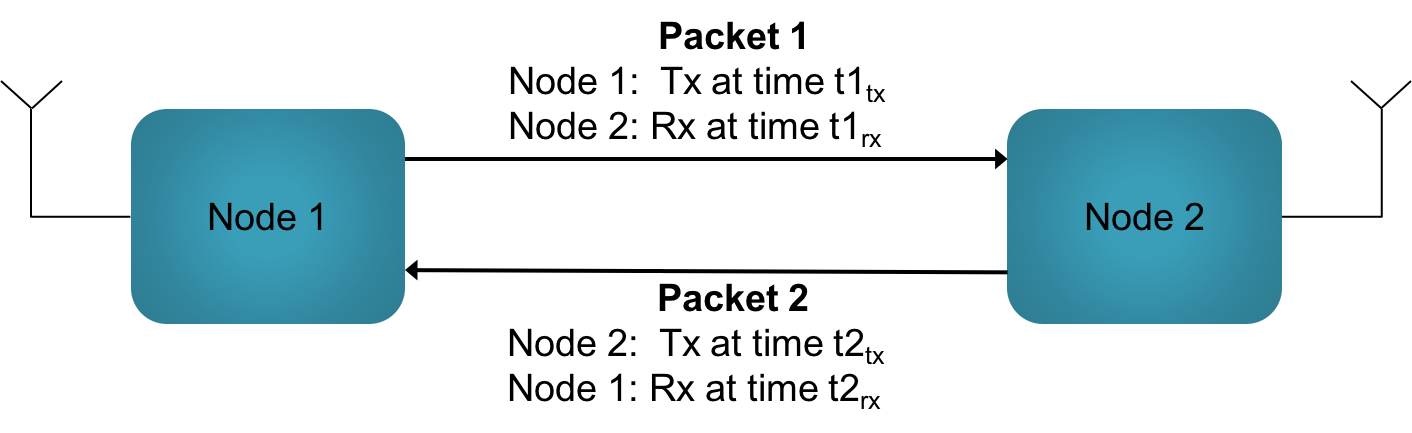
\includegraphics[width=3.5in]{tof.png}
\caption{{Illustration of Time of Flight algorithm}}
\label{fig:tof}
\end{figure}
\begin{equation}
\label{eq:tof}
    T = (t2_{rx} - t1_{tx}) - (t2_{tx} - t1_{rx})
\end{equation}

\begin{equation}
\label{eq:distcalc}
    Distance = \frac{Speed\ of\ Light \times T}{2}
\end{equation}

\subsubsection{Time Difference of Arrival}
The time-difference-of-arrival (TDOA) method is comparitively a more scalable algorithm for localization.  In this method, the target tag periodically sends beacons to anchors in its vicinity.  When the anchors have time synchronized clocks, the time difference of arrival of the packet at between each pair of anchor nodes defines a hyperbolic surface on which the target tag must lie.  The tag's 3D location can be computed by finding the intersection of all these hyperbolic surfaces. However, it does require very precise time synchronization between the clocks of every anchor in the network\cite{mcelroy2014comparison}.  Specifically for the DWM1000, the medium is an electromagnetic wave, so any error in time synchronization gets multiplied by the speed of light.  We chose to start our implementation with the TOF method because it is much simpler to implement and the DWM1000's factory calibration takes care of a lot of the error-causing factors that the TOF method is susceptible to.  While we did keep TDOA as a stretch goal, our primary objective was still to get the entire system up and running with the best possible accuracy achievable with TOF since time-synchronizing all these wireless nodes is a hard problem. 


\subsection{System Architecture}
The goal of the project was to implement a system which achieves high 3D localization accuracy and low enough power consumption to be powered by a Li-Ion battery.  We used Time-of-Flight to measure the distance of the tag node with respect to each one of the anchor nodes and then used a WiFi network to transmit the distance data from the tag to the backend software running on a PC.  The PC runs a Python script to connect to the mobile node and collects the distance data with Anchor ID.  This data is then processed by a series of signal processing steps (described in section \ref{sec:impl}) to localize the target and give the user an intuitive and interactive graphical output about the tag's location. Decawave claims a 1D distance measurement accuracy of $\approx$10cm using these sensors.  After calibration, we acheived a best case accuracy of $\approx$10cm on all 3 dimensions, and an average accuracy of $\approx$20cm on all 3 dimensions, which is at par with the device manufacturer's claims. \\

The 3D location of any node can be found if the distance from four anchor nodes of fixed location in 3D space is known.  In the TOF method, for example, the distance "d" from one anchor node defines a sphere with radius "d" around that node.  The surface of this sphere is the locus of points where the tag must lie.  The spheres formed by the distances from two anchors intersect at a circle, the perimeter of which is the locus of points where the tag must lie.  A third anchor generates another sphere which meets this circle at two possible points.  A fourth anchor is needed to find which of these points the tag must lie in.  Ofcourse, in real world systems, there is a finite measurement error, and none of these spheres are clearly defined.  Therefore, a closed form solution of the system of equations formed by these four spheres may not exist all the time.  Therefore, a least-squares equation solver is used to minimize the set of equations and find the most probable location of the tag. The system setup of our system is shown in Figure \ref{SYSTEMBD} with three anchor nodes.\\
\begin{figure}[!h]
\centering
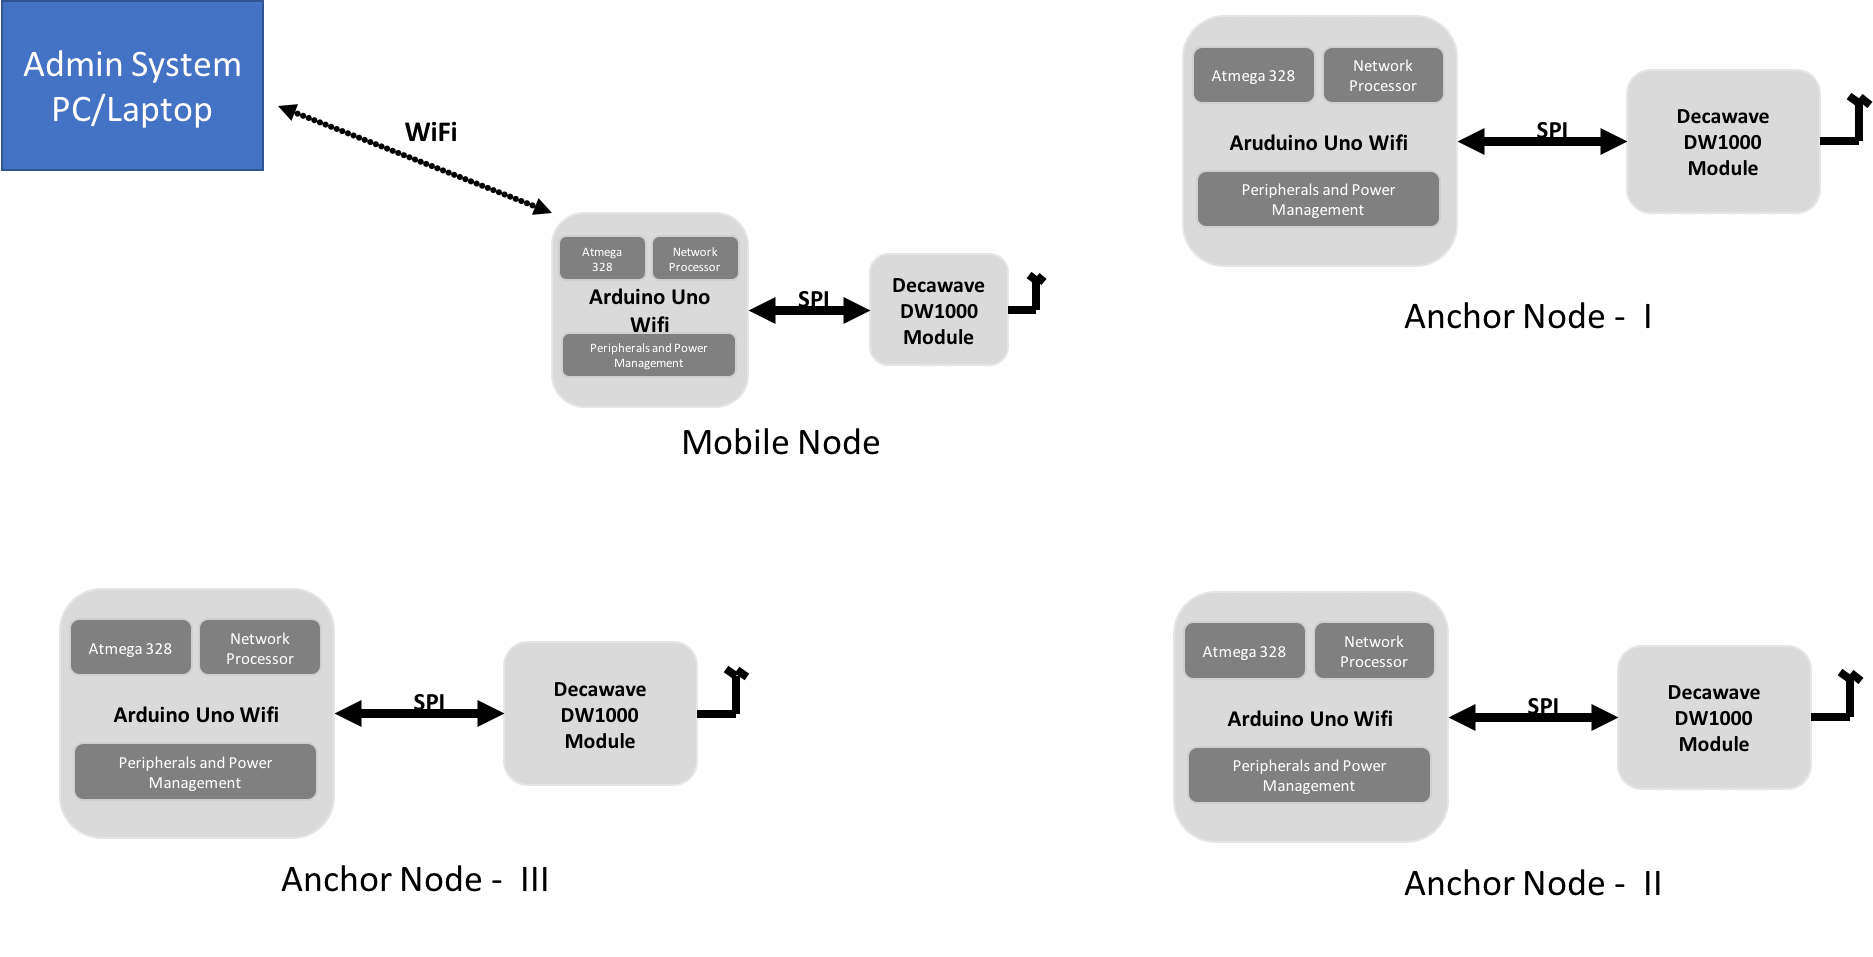
\includegraphics[width=3.5in]{sysbd.png}
\caption{{Complete system architecture}}
\label{SYSTEMBD}
\end{figure}
To obtain the distance measurements, we use time of flight of radio waves over the UWB spectrum. The DWM1000 sends very short chirps of radio signals in the UWB spectrum. The benefits of this include a very fine time resolution, energy efficiency, and most importantly, robustness to interference in harsh environments \cite{uwb}. UWB is also particularly resilient to multi-path fading effects.  In this project, we use the Decawave ScenSor DWM1000 Modules for UWB TOF measurements. Using these modules the distance of the mobile node from each of the anchor nodes is determined. This information is accumulated at a gateway for the multilateration computation. For this we interface DWM1000 with Arduino Uno Wifi using the SPI interface supported by DWM1000. 

\subsection{Software Design}

\subsubsection{Backend Software}
Python was chosen as the language for backend computation for the following reasons:
\begin{itemize}
    \item Scipy and Numpy packages provide ready access to minimization functions required for localization algorithm
    \item Matplotlib package provides an environment to scatter plot the tag location in 3D
    \item Python being a high level language is best suited for prototyping. The tradeoff in speed was tolerable in this application as the point did not have to be plotted in realtime.
    \item Availability of Telnet library to connect to the Tag listening socket and read the distance values.
\end{itemize}
\subsubsection{Decawave Library}
The Arduino DWM1000 library hosted by Thomas Trojer on github was used\cite{thotro:2017}. This library had the 2 way ranging code implemented with instructions on how to interface the DWM1000 with the Arduino. The library was still active as of writing this report.

\subsubsection{WiFi Library}
The standard library which ships with Aruduino Uno Wifi was used. It came with a reference program to relay the serial readings over Wifi. This library also makes the Arduino Uno a WiFi access point. The advantage of this compared to connecting to a public access point was the static IP allocation of the Tag node. Since the Tag was hosting the access point it always had the first IP in the subnet eliminating the need for having access to the public DHCP server.

\subsection{Hardware Design}
\subsubsection{Micro-controller Platform Decision}
When we initially started the project we had a set of specifications in mind for the microcontroller and wireless communication device.  We required a low power microcontroller board with low power WiFi connectivity.  The MCU should have at least one SPI and one UART port for interfacing with the Decawave and debugging in addition to whatever interface it requires for WiFi.  One solution was to use a low power MCU platform like Arduino or TI's MSP430/432 Launchpad and an external WiFi board like the Arduino WiFi sheild or the CC3100 BoosterPack.  However, we already had a Decawave board and a set of level shifter ICs and we did not want to add an additional board (and therefore another point of failure).  We then refined our requirement and looked for single board solutions that incorporated a WiFi radio along with a low power MCU.  While the Raspberry Pi is an obvious solution to this, we decided against it since the Raspberry Pi comes with a 1GHz ARM processor and high speed WiFi radio, both of which were an overkill for this application and had a power consumption that was definitely out of budget.  Finally, we narrowed down to the CC3200 Launchpad and the Arduino UNO WiFi.  We initially selected the CC3200 since it incorporates a single chip WiFi+MCU and we thought its power consumption would be lower, and the powerful 80MHz ARM Cortex M4 on the CC3200 might be needed for our algorithms.  However, upon carefully analyzing our options, we concluded in favor of the Arduino for the following reasons:\\

\textit{Library Support:}
The Decawave SPI driver and 1D ranging libraries were readily available for Arduino platforms and not directly available for the CC3200.  While the CC3200 does support the "Arduino-like" Energia platform, significant porting effort may have been needed just to get the CC3200 to talk to the Decawave.  The Arduino was preferable since the Arduino SPI libraries take care of the hardware abstractions and board-to-board dependencies.\\

\textit{On-chip Flash:}
The CC3200 also suffers from another drawback, which is the fact that it does not come with any on-chip flash.  While this is taken care of in the launchpad with the help of an external flash on the board, an MCU with on-chip flash benefits from easier programming and deployment.  We saw this as a major concern for the later stages of the the project where we would need to test and calibrate multiple of these boards and program them to make tweeks during testing time.  It is more convenient to have a device with built-in flash rather than requiring the additional step of using TI's UNIFLASH to program the external flash on the CC3200 board.\\

\textit{Power consumption:}
The CC3200 has an active power consumption of about 15.3mA at 3.3V without the WiFi radio on, which translates to an active power consumption of 50.49mW. When the WiFi radio is active at peak power, the total current consumption is 278mA at 3.3V, which is 917.4mW of peak active power excluding the power consumption of the external flash, which draws an additional standby current during runtime.
The ATMega328P consumes about 5.2mA at 5V when active, which translates to about 26mW active power consumption.  We needed to use 2 Arduinos in order to not stress the RAM on a single Arduino and obtain stable operation.  Therefore, the combined power consumption of both Arduinos is 52mW.  The Arduino responsible for WiFi transmission was an Arduino UNO WiFi with an ESP8266 WiFi Radio. The ESP8266 WiFi SoC on the Arduino UNO WiFi board has a peak power consumption of 170mA at 3.3V, and therefore has a peak power consumption of 561mW.  Therefore, our combined active power consumption for the 2 Atmel microcontrollers along with the ESP8266 is 613mW.  This makes the combined Arduino solution about 33\% more power efficient than the CC3200 solution, even without considering the CC3200's external flash's standby current. \\
\begin{figure}[!h]
\centering
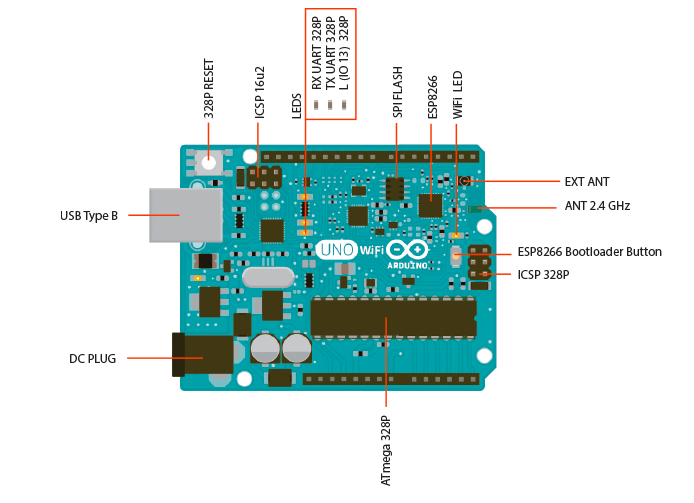
\includegraphics[width=2.5in]{arduinounobd}
\caption{{Board layout of Arduino Uno Wifi SoC}}
\label{arduinoBD}
\end{figure}
The main reason for choosing the CC3200 initially was that we were able to get a powerful MCU and a WiFi chip in a low cost, low power board.  However, we realized that it was more suitable to run the math-heavy least-squares linear equation solver needed for accurate localization on the backend software on a PC.  This gives us more flexibility to use the vast collection of mathematical libraries and filters available in NumPy while also reducing our MCU's CPU utilization.  Since we no longer needed such a powerful MCU, the Arduino's processing power and memory was sufficient for our purposes.  Based on the above reasons, we concluded that the Arduino UNO WiFi was the right device for the job. The block diagram of Arduino UNO WiFi is shown in Figure \ref{arduinoBD}\\
\begin{figure}[!h]
\centering
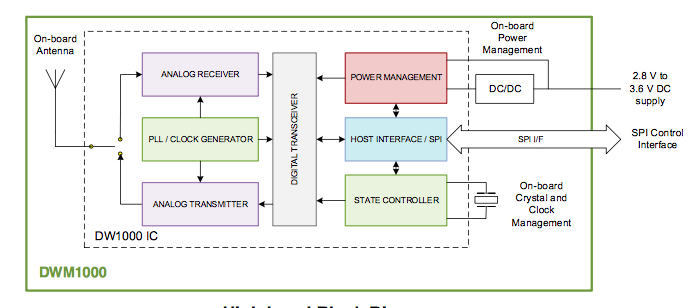
\includegraphics[width=3.5in]{dw1000bd}
\caption{{Block Diagram of DW1000 UWB transceiver}}
\label{DW1000BD}
\end{figure}
\subsubsection{DWM1000 Module}
Due to the advantages mentioned in the previous sections, using a UWB based sensor helps us achieve better accuracy and also avoid multi-path fading. DWM1000 modules from Decawave claim an accuracy of $\approx$10cm between two nodes. DWM1000 modules are sensors which use DW1000 chips with RF and clock circuitry. The modules can be interfaced over SPI and requires a 3.3V external power supply. The block diagram of DWM1000 module is shown in Figure \ref{DW1000BD}. Time-of-flight applications are sensitive to clock drifts which can reduce the accuracy significantly. To alleviate the effect of clock drifts, the clocks on the modules are factory trimmed to within +/- 2ppm under typical conditions. Due to the reasons stated above, DWM1000 matches with our requirement. Other advantages of using DWM1000 modules are listed below:
\begin{itemize}
	\item Upto to 6.8Mb/s achieved in Wireless Sensor Networks
	\item Communication range of upto 290m
	\item Low power consumption
	\item Compact size
	\item RF design is not required
	\item Integrated antenna
\end{itemize}

Each node (both tag and anchors) have Arduino UNO WiFi board and a Decawave module interfaced over SPI. The hardware architecture of each node is shown in Figure \ref{EACHNODEBD}
%Describe why CC3200.
\begin{figure}[!h]
\centering
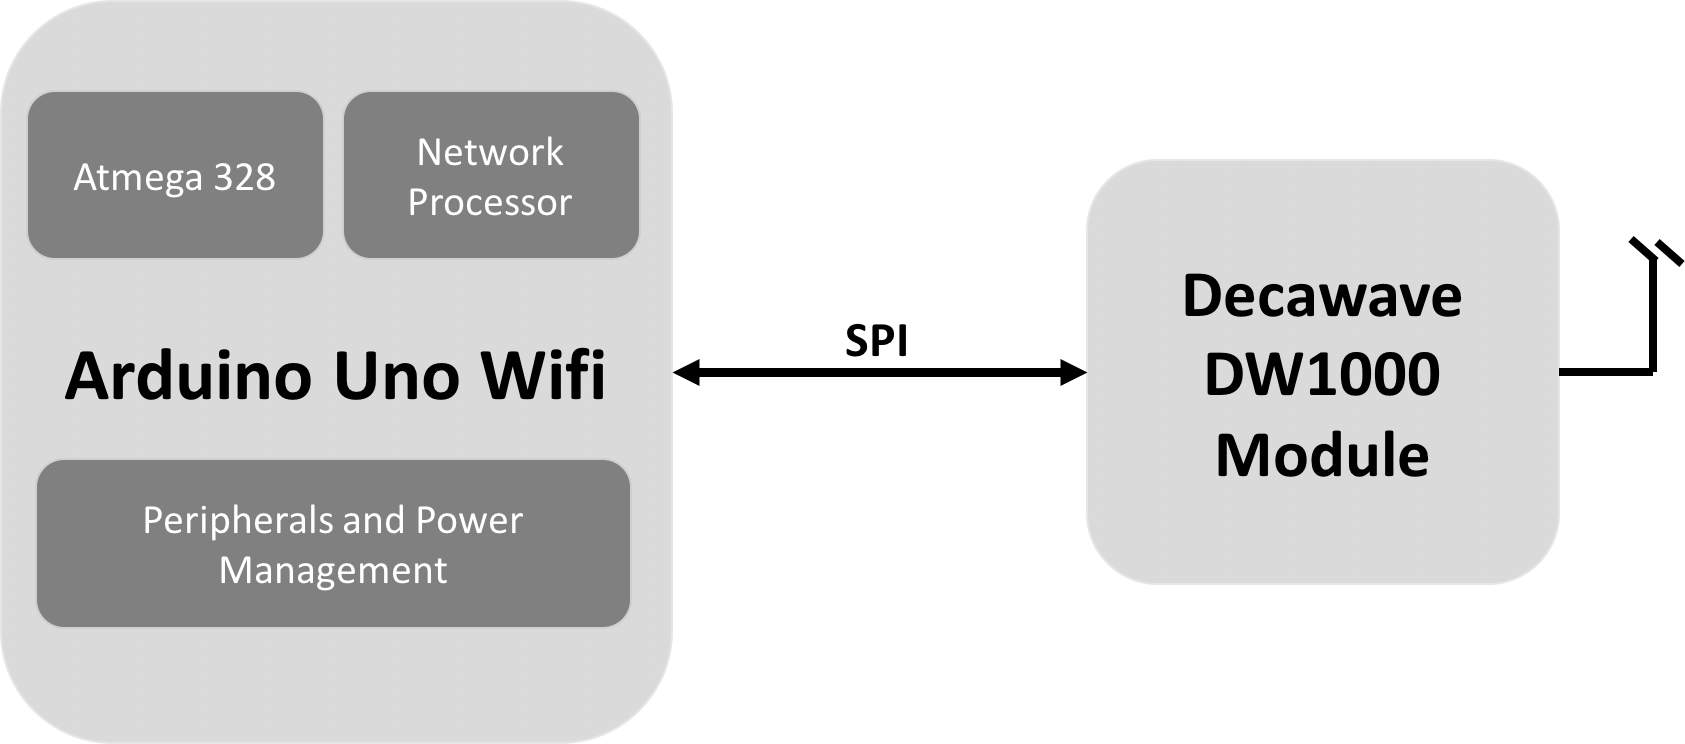
\includegraphics[width=3.5in]{nodebd.png}
\caption{{System Block Diagram of Each Node}}
\label{EACHNODEBD}
\end{figure}




%One disadvantage of using ToF algorithm is that it cannot be scaled. As the number of nodes increase, we expect each node to consume more energy. As an extended goal, we propose to use Time Difference of Arrival(TDOA)\cite{anthonyrowe's paper} to provide scalability. In this system architecture, anchor nodes will broadcast their location to all the nodes that are being localized in the vicinity. Using the anchor node's location and the difference in time of arrival of packets from each of the anchor nodes, triangulation can be performed. A detailed explanation of these algorithms are provided in the next section.

\section{Implementation}\label{sec:impl}
As shown in figure \ref{SYSTEMBD}, we use multiple anchor nodes with known positions to locate a mobile node. We use dynamic network discovery to connect tags with anchor nodes and perform 2-way ranging with each anchor node. The calculated distance between the tag and each anchor is sent from the tag to an admin laptop over WiFi. The distances from four anchor nodes is used to perform localization. The error of localization in our implementation is as low as \textbf{10 cm on each axis} in the best case. On an average, we are able to locate the mobile node \textbf{within 20 cm on all three axes}. 

\subsection{Network Discovery and Communication}
A mobile tag node performs network discovery and initiates 2-way ranging with each of the anchor nodes. \textit{TAG} node controls the entire network to calculate the point-to-point distances between the anchor nodes and itself. As soon as the \textit{TAG} node is turned on, it broadcasts a \textbf{POLL} packet to all its neighbours. All the \textit{ANCHOR} nodes that receive the broadcast packet, respond with a \textbf{POLL\_ACK} message. The mobile node uses these acknowledgement messages to prepare a list of anchor nodes in its range. It is important to note that the mobile node sends one broadcast message and receives multiple acknowledgment messages.\\  
\begin{figure}[!h]
\centering
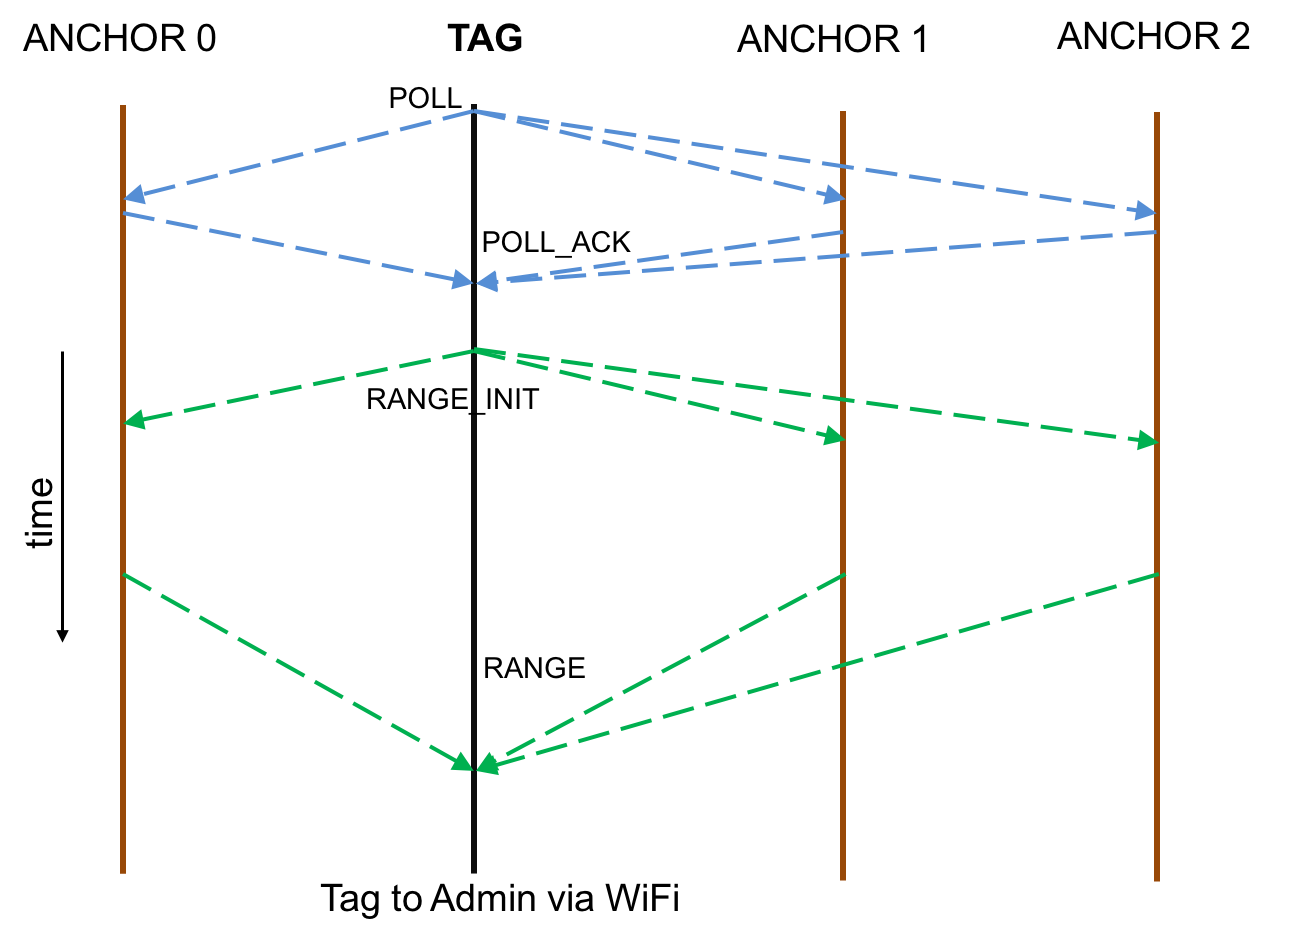
\includegraphics[width=3.5in]{communication.png}
\caption{{Network discovery and two-way ranging protocol}}
\label{commsystem}
\end{figure}
Using the network discovery performed using \textbf{POLL} and \textbf{POLL\_ACK} messages, the mobile node maintains a list of anchor nodes and performs 2-way ranging with each of those nodes. Once the anchor nodes respond with \textbf{POLL\_ACK} message, it waits to receive the \textbf{RANGE\_INIT} packet from the mobile node. \textbf{RANGE\_INIT} and \textbf{RANGE} packets are exchanged between the nodes using timestamps to perform 2-way ranging. As shown in figure \ref{commsystem} the messages exchanged between the mobile node and the anchor nodes involve multiple steps and are performed one after the other. 

If an anchor node goes out of range after responding with the acknowledgement message, the mobile node marks it as an inactive node and deletes the corresponding anchor node from its network list. Thus, our communication protocol can discover dead anchor nodes immediately.

\subsection{Ranging Calibration}
Although the timestamps used by DWM1000 modules to perform 2-way ranging are quite accurate, there is an error in the point-to-point distance calculated due to the communication protocol overhead. Comparison between the actual distance and the calculated distance was made. It is observed that for small ranges, the percentage error in the distance measurement is quite high and this error reduces as the distance between two nodes increase. The error is calculated for distances from few centimeters to 10 meters and the plot is shown in figure \ref{abs_error} \& \ref{errorcalib}. 
\begin{figure}[!h]
\centering
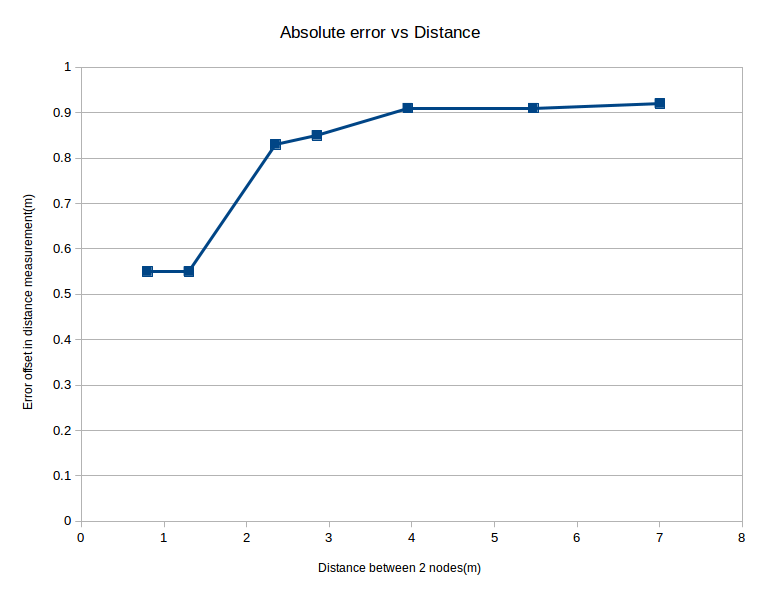
\includegraphics[width=3.5in]{wsn_abs_error.png}
\caption{{Absolute error between 2 nodes while doing 2-way ranging}}
\label{abs_error}
\end{figure}

\begin{figure}[!h]
\centering
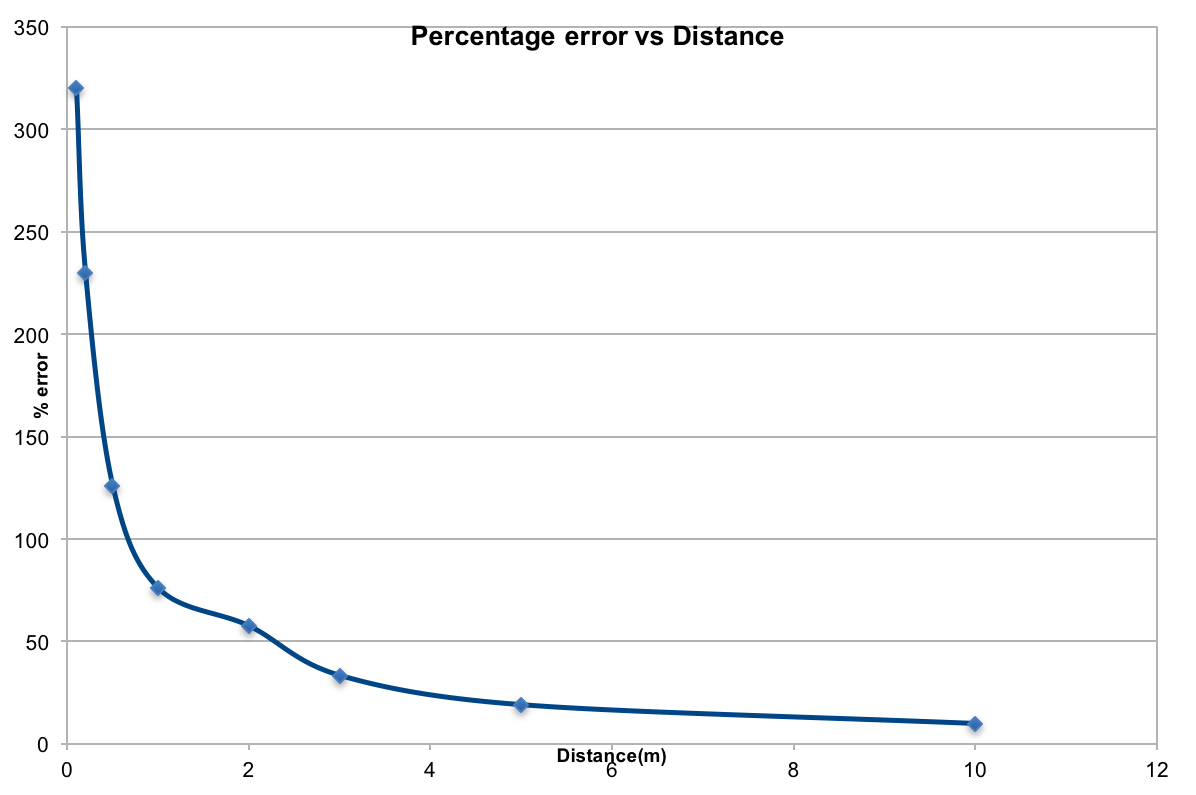
\includegraphics[width=3.5in]{errorcalibfig.png}
\caption{{Percentage error between 2 nodes while doing 2-way ranging}}
\label{errorcalib}
\end{figure}

We use this data to calibrate the ranges sent from mobile node to the admin laptop. The point-to-point distance between the tag node and each anchor node is calibrated using a piecewise linear look-up table. Error calibration using this technique increased the localization accuracy significantly. The error calibration increased the accuracy from 50 cm on all three axes to 20 cm on an average. This also made our equation solver stable and converge sooner.
\subsection{Localization}
The equations for localization were solved in Python using the Localization library\cite{kamalshadi:2017}. This library uses SciPy and NumPy libraries to find a least square error estimate of the three co-ordinates. The total error was defined as shown in Equations \ref{eq:error} and \ref{eq:dist}
\begin{equation}
\label{eq:dist}
D_i = \sqrt{(X-x_i)^2 + (Y-y_i)^2 + (Z-z_i)^2}
\end{equation}
where, $D_i$ is the distance of the tag from anchor $i$.\\
\begin{equation}
\label{eq:error}
 error = \sum\limits_{i} (D_i - r_i)^2 \forall\ anchor\ i
\end{equation}
where, $r_i$ is the range measured by DWM1000 to anchor $i$.\\

This error was minimized using $scipy.optimize.minimize$ with the initial estimate $X=0,Y=0,Z=0$.

\begin{figure}[!h]
\centering
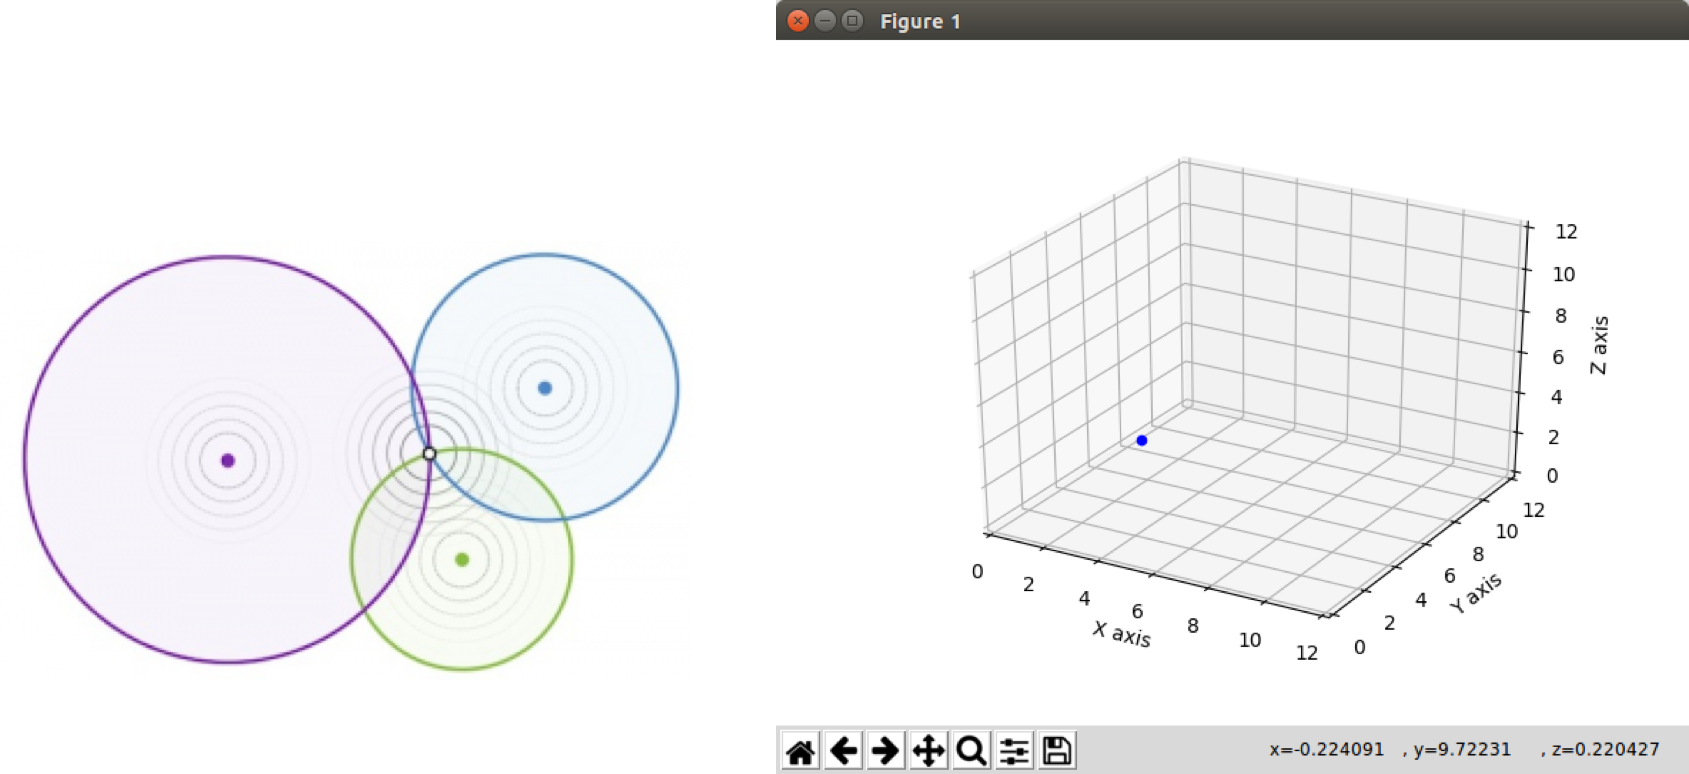
\includegraphics[width=3.5in]{3D_localization.png}
\caption{{3-D Localization}}
\label{3dlocalization}
\end{figure}

Further information on the equations used and the corresponding equations for TDOA can be found in \cite{gaffney2008considerations}



\subsection{Placement of Anchor Nodes}

Different cofigurations of placement of anchor nodes was tried out. When all four anchor nodes were placed in one plane, the error in distances from each anchor gets compounded along the perperdicular dimension. Therefore the best possible placement was achieved by placing the 4 anchors as orthogonal as possible as shown in Figure: \ref{anchorplacement}. The lengths along each dimension were chosen for convenience of placing anchor nodes.


\begin{figure}[!h]
\centering
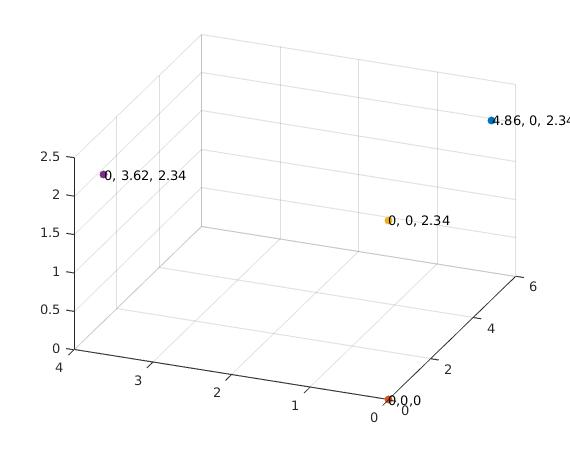
\includegraphics[width=3.5in]{anchorplacements3d.jpg}
\caption{{Placement of four Anchor Nodes. All dimensions are in meters.}}
\label{anchorplacement}
\end{figure}



\subsection{Median Filtering}

To eliminate noise iin the samples, median filtering was performed on a sliding window. Median is particularly resilient to sparse errors. Hence the last 5 calculated co-ordinates were held in a queue. The present co-ordinate was chosen to be the median of these 5 values. This made our co-ordinates very robust.


\begin{figure}[!h]
\centering
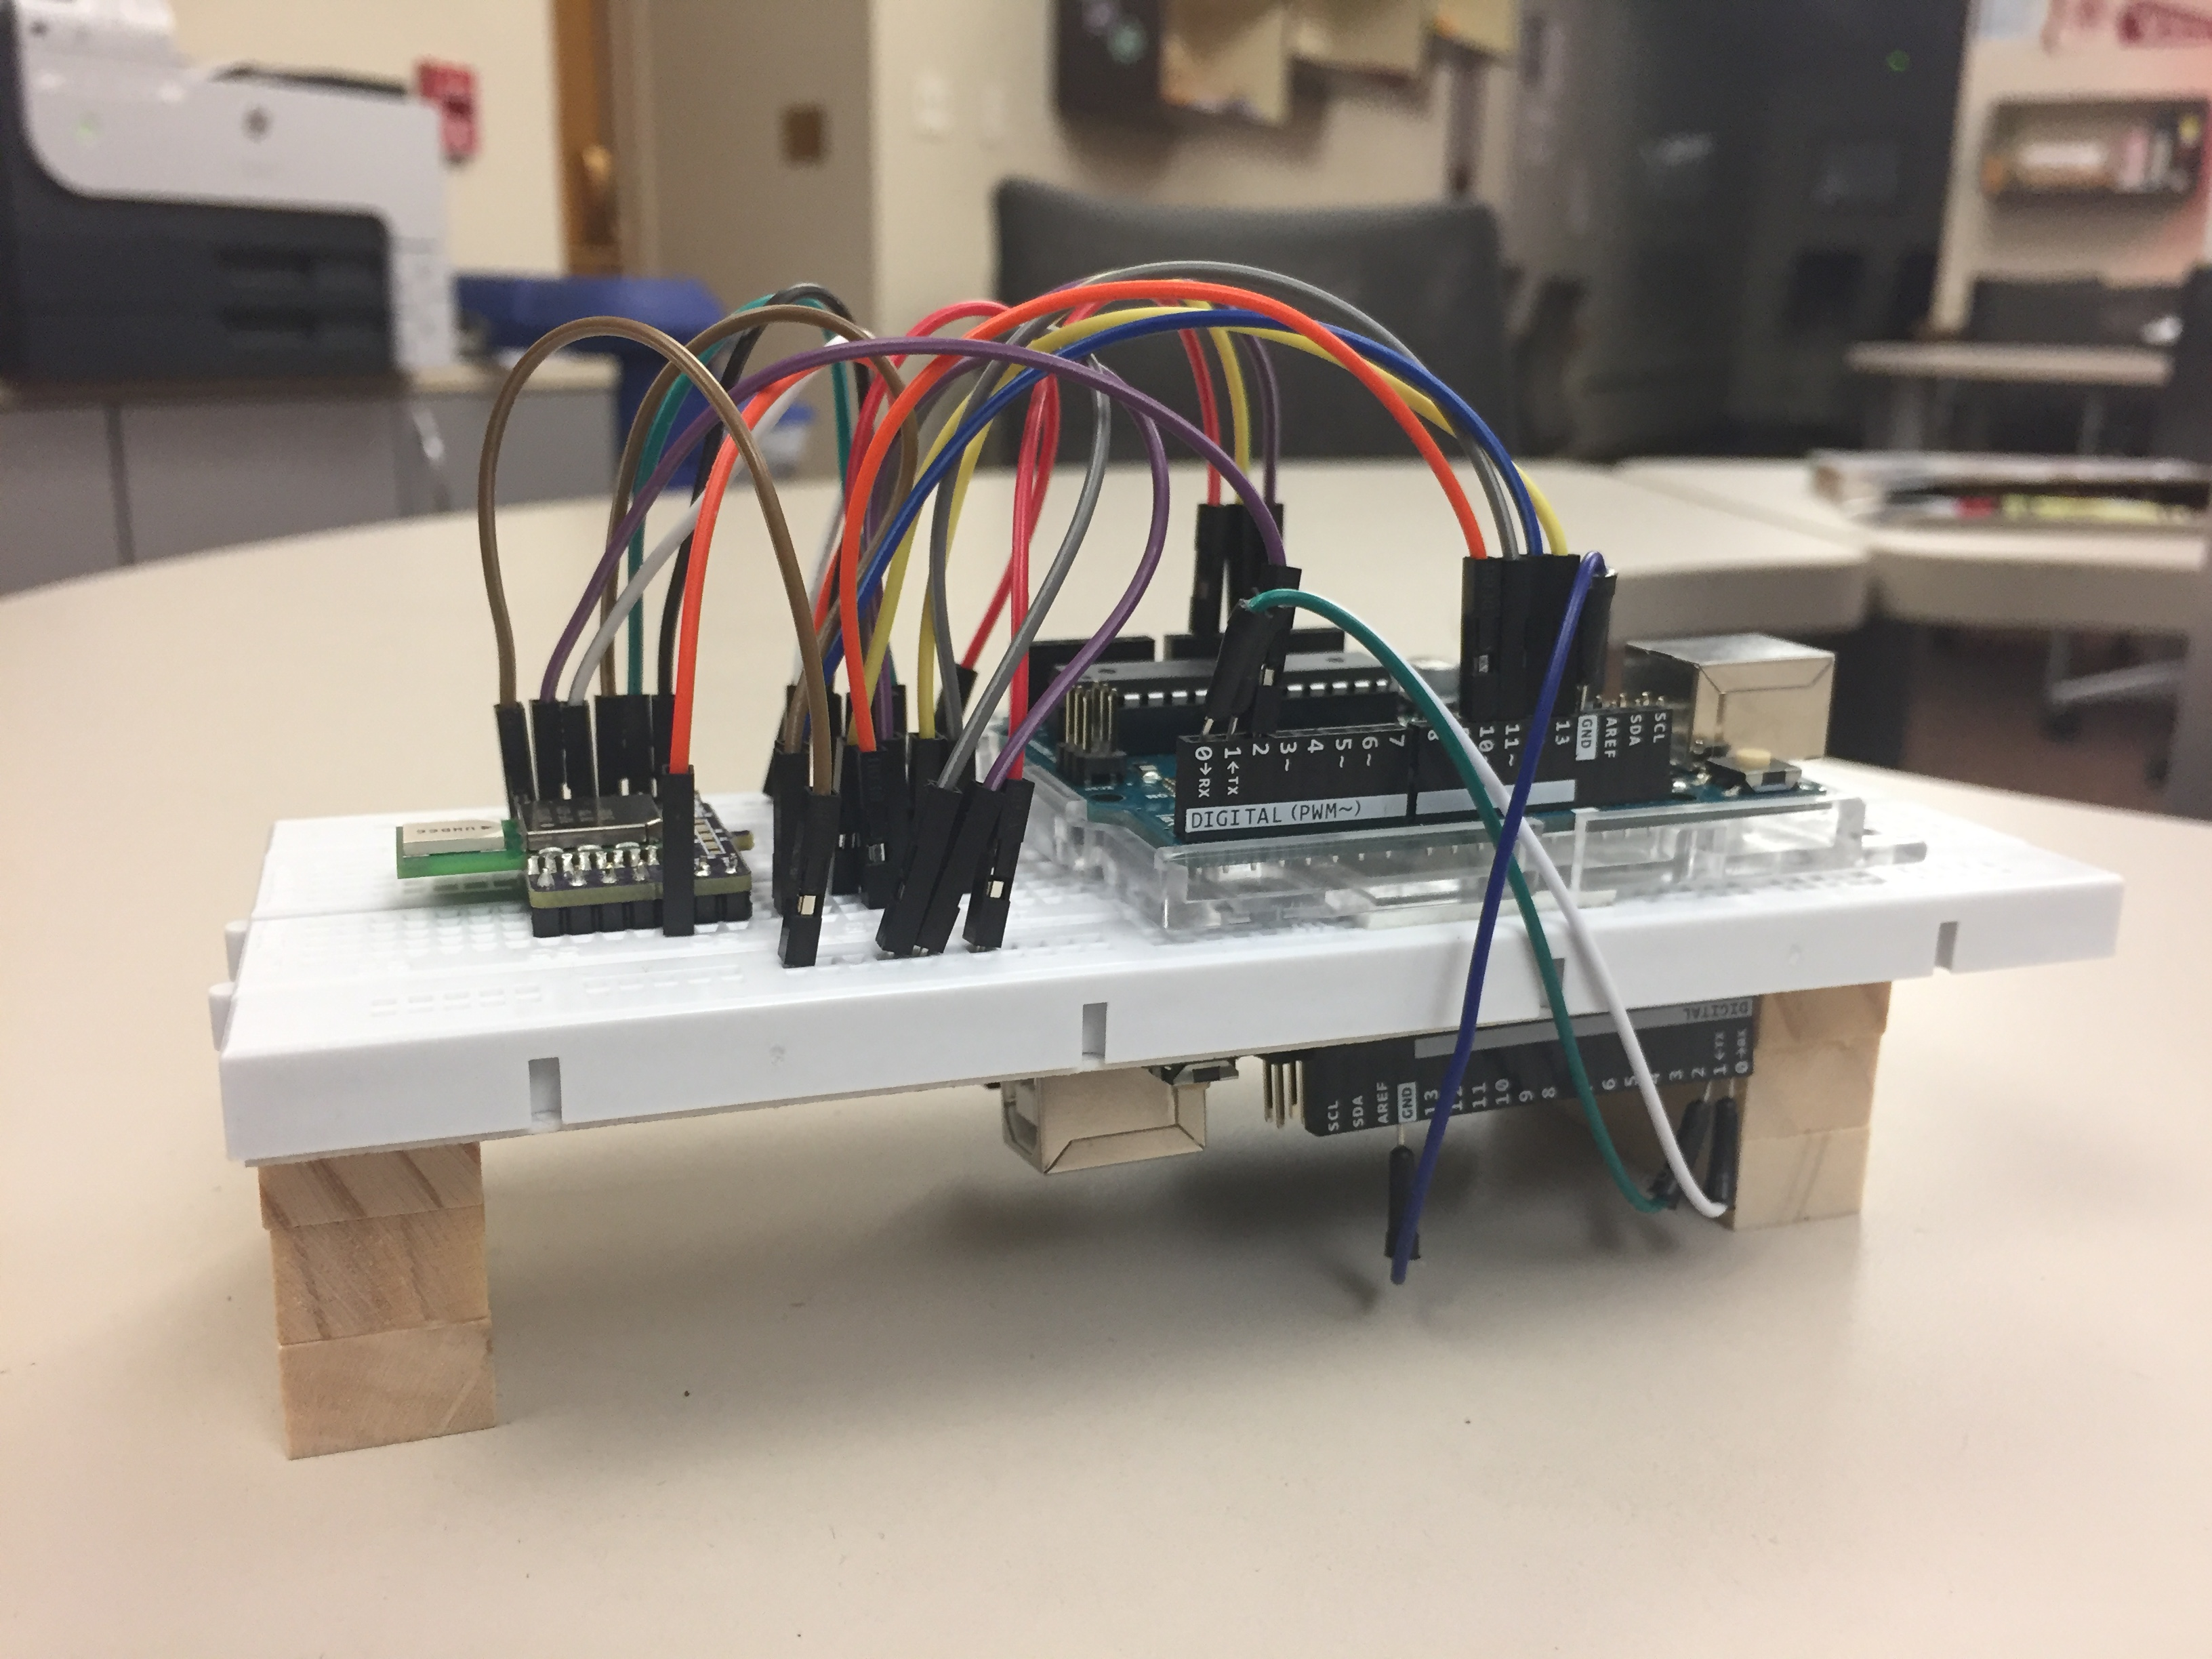
\includegraphics[scale=0.075]{tagnode.JPG}
\caption{{TAG node: DWM1000 and Arduino on top; Arduino UNO Wifi is mounted on the bottom}}
\label{fig:tagnode}
\end{figure}

\section{Challenges}
We faced a number of challenges during the course of this project.  These are listed below: 

\begin{itemize}
\item DWM1000 did not come with a base board to mount on a breadboard. This base board was ordered separately.
\item DWM1000 works on 3.3V while the Arduino Uno works on 5V. We had to procure level shifters to downshift the required SPI lines.
\item The library for 2-way ranging was not stable with more than 2 anchors. These were identified as arising due to race conditions in the library code. After considerable probing, we were able to narrow down the bug to the variable whose access was shared.
\item The distance measurements given by DWM1000 was initially off by about 1m. After plotting the actual distance vs the distance measured by DWM1000, it was evident that there is an offset between the two values. These offsets were recorded for each piecewise interval. A function was written which would convert the uncalibrated distance measured by DWM1000 to the actual distance by subtracting the corresponding offset.
\item The Arduino Uno board did not have enough RAM to run both the ranging code as well as the WiFi library. The workaround for this problem was to attach another Arduino to act as a WiFi network processor for the tag. This Arduino would receive the ranging distance value over UART and transmit the data over WiFi.
\item The addition of another slave Arduino for WiFi relaying brought in additional constraints in keeping the Tag physically small and concise. We had to design custom legs for the breadboard to house both the Arduinos without bloating the Tag dimensions.
\end{itemize}
\section{Future Work}
Our system can be improved further which are mainly based on the challenges we faced during our implementation stage. 
The current system is tested with a single mobile node and four anchor nodes. The system can be tested with multiple mobile nodes to check the performance. However, we believe that the four anchor nodes will not be able to service the range requests from multiple tag nodes, resulting in inaccurate ranges and delayed localization. \\

The current solution uses a two board approach to provide connectivity to the localization system over WiFi. This is mainly due to the limited RAM available on the Arduino boards. The DWM1000 library can be ported to a more powerful SoC like CC3200 to achieve a one board solution. With a more powerful SoC like CC3200, the localization equation solving can be done on the SoC itself. This eliminates the need for a separate computation backend server.\\

Time-Difference-of-Arrival algorithm can be used to perform localization with multiple mobile nodes. This will reduce the load on the anchor nodes. We expect this system to be more scalable as the number of mobile nodes increase. However, this approach requires accurate time synchronization between the mobile nodes. For time synchronization \cite{mcelroy2014comparison} proposes few methods which involve a master anchor transmitting clock synchronization packets every fixed interval. This packet is used by the other slave anchors to synchronize their time with the master anchor node. We also propose an iterative process to synchronize the clocks by localizing the 4th anchor(known co-ordinates) using the other 3 and changing the clock skews to increase the localization accuracy in every iteration.\\

Our system currently requires measuring the precise locations of the anchors and programming it into the Tag before the deployment of the system. A SLAM inspired approach can be taken wherein the user can place the anchors around the room. The Tag then guides the user to different landmarks around the room. This information is then used to learn the dimensions of the room. This approach is demonstrated and further elucidated in \cite{alps}.\\

Security is another aspect that must be considered for real world deployment. A malicious agent must not be able to know the location of the Tag. This will require encrypting the messages transferred between the anchor and the tags.\\

\section{Conclusion}
In conclusion, with our design choices and system architecture, our system is able to perform localization of mobile nodes in an indoor environment successfully. Our implementation is a completely self sufficient system and makes no assumptions regarding the availability of WiFi, internet or power source. Therefore the system can be used to perform localization in any indoor setting. A key observation from this project is that placement of anchor nodes have a significant effect on the accuracy of the system. We have achieved a best case accuracy of 10cm and 20cm accuracy on an average. Figure \ref{fig:tagnode} shows our final Tag assembly.
\section{Milestones}
The following were the key milestones during the course of the project:
\begin{center}
\begin{tabular}{ |m{1.5cm}|m{6.0cm}|}
\hline
\textbf{Week} & \textbf{Progress} \\ 
\hline
Mar 27-31 & Basic Arduino Code test, Solder 2x DW1000
modules, breadboard prototyping, Python interface\\
\hline
Apr 3-7 &Mid term demo. Level shifters interface, DW1000
baseboards arrive, Tag and anchor nodes bring up\\
\hline
Apr 10-14 & Develop TOF code with 5 DW1000 modules
working at once\\
\hline
Apr 17-21 & Change library for robust multi-anchor network
connectivity and addressing\\
\hline
Apr 24-28 & Test TOF Code with 4 anchor+1 tag. Accuracy
measurements,
integrating solver code with python interface code
and GUI extension\\
\hline
May 1-5 & Prep for final demos, code and H/W cleanup,
calibrations, WiFi Integration\\
\hline
\end{tabular}
\end{center}



\section{Work Partitioning}
The work was divided between the team members as follows:

\begin{center}
\begin{tabular}{ |m{6cm}|m{1.25cm}|}
\hline
Work Items &	Team Member\\
\hline
Python UI, data processing/Algorithm, socket programming for WiFi connection, DWM1000 offset calibration, Arduino-DWM1000 library bug fixes&	Tejus\\
\hline
Embedded programming - DWM1000 Interface, TOF Algorithm, DWM1000 offset calibration, Anchor placement tuning &	Albert\\
\hline
Embedded Programming - WiFi Chip Interface, Data Transfer to PC Over WiFi, Arduino-DWM1000 library bug fixes & Anirban\\
\hline
Board bring up, HW interface, other setup & All\\
\hline
\end{tabular}
\end{center}

\pagebreak


% An example of a floating figure using the graphicx package.
% Note that \label must occur AFTER (or within) \caption.
% For figures, \caption should occur after the \includegraphics.
% Note that IEEEtran v1.7 and later has special internal code that
% is designed to preserve the operation of \label within \caption
% even when the captionsoff option is in effect. However, because
% of issues like this, it may be the safest practice to put all your
% \label just after \caption rather than within \caption{}.
%
% Reminder: the "draftcls" or "draftclsnofoot", not "draft", class
% option should be used if it is desired that the figures are to be
% displayed while in draft mode.
%
%\begin{figure}[!t]
%\centering
%\includegraphics[width=2.5in]{myfigure}
% where an .eps filename suffix will be assumed under latex, 
% and a .pdf suffix will be assumed for pdflatex; or what has been declared
% via \DeclareGraphicsExtensions.
%\caption{Simulation results for the network.}
%\label{fig_sim}
%\end{figure}

% Note that the IEEE typically puts floats only at the top, even when this
% results in a large percentage of a column being occupied by floats.


% An example of a double column floating figure using two subfigures.
% (The subfig.sty package must be loaded for this to work.)
% The subfigure \label commands are set within each subfloat command,
% and the \label for the overall figure must come after \caption.
% \hfil is used as a separator to get equal spacing.
% Watch out that the combined width of all the subfigures on a 
% line do not exceed the text width or a line break will occur.
%
%\begin{figure*}[!t]
%\centering
%\subfloat[Case I]{\includegraphics[width=2.5in]{box}%
%\label{fig_first_case}}
%\hfil
%\subfloat[Case II]{\includegraphics[width=2.5in]{box}%
%\label{fig_second_case}}
%\caption{Simulation results for the network.}
%\label{fig_sim}
%\end{figure*}
%
% Note that often IEEE papers with subfigures do not employ subfigure
% captions (using the optional argument to \subfloat[]), but instead will
% reference/describe all of them (a), (b), etc., within the main caption.
% Be aware that for subfig.sty to generate the (a), (b), etc., subfigure
% labels, the optional argument to \subfloat must be present. If a
% subcaption is not desired, just leave its contents blank,
% e.g., \subfloat[].


% An example of a floating table. Note that, for IEEE style tables, the
% \caption command should come BEFORE the table and, given that table
% captions serve much like titles, are usually capitalized except for words
% such as a, an, and, as, at, but, by, for, in, nor, of, on, or, the, to
% and up, which are usually not capitalized unless they are the first or
% last word of the caption. Table text will default to \footnotesize as
% the IEEE normally uses this smaller font for tables.
% The \label must come after \caption as always.
%
%\begin{table}[!t]
%% increase table row spacing, adjust to taste
%\renewcommand{\arraystretch}{1.3}
% if using array.sty, it might be a good idea to tweak the value of
% \extrarowheight as needed to properly center the text within the cells
%\caption{An Example of a Table}
%\label{table_example}
%\centering
%% Some packages, such as MDW tools, offer better commands for making tables
%% than the plain LaTeX2e tabular which is used here.
%\begin{tabular}{|c||c|}
%\hline
%One & Two\\
%\hline
%Three & Four\\
%\hline
%\end{tabular}
%\end{table}


% Note that the IEEE does not put floats in the very first column
% - or typically anywhere on the first page for that matter. Also,
% in-text middle ("here") positioning is typically not used, but it
% is allowed and encouraged for Computer Society conferences (but
% not Computer Society journals). Most IEEE journals/conferences use
% top floats exclusively. 
% Note that, LaTeX2e, unlike IEEE journals/conferences, places
% footnotes above bottom floats. This can be corrected via the
% \fnbelowfloat command of the stfloats package.



% if have a single appendix:
%\appendix[Proof of the Zonklar Equations]
% or
%\appendix  % for no appendix heading
% do not use \section anymore after \appendix, only \section*
% is possibly needed

% use appendices with more than one appendix
% then use \section to start each appendix
% you must declare a \section before using any
% \subsection or using \label (\appendices by itself
% starts a section numbered zero.)
%





% trigger a \newpage just before the given reference
% number - used to balance the columns on the last page
% adjust value as needed - may need to be readjusted if
% the document is modified later
%\IEEEtriggeratref{8}
% The "triggered" command can be changed if desired:
%\IEEEtriggercmd{\enlargethispage{-5in}}

% references section

% can use a bibliography generated by BibTeX as a .bbl file
% BibTeX documentation can be easily obtained at:
% http://mirror.ctan.org/biblio/bibtex/contrib/doc/
% The IEEEtran BibTeX style support page is at:
% http://www.michaelshell.org/tex/ieeetran/bibtex/
\bibliographystyle{IEEEtran}
% argument is your BibTeX string definitions and bibliography database(s)
%\printbibliography
\bibliography{refer}
%
% <OR> manually copy in the resultant .bbl file
% set second argument of \begin to the number of references
% (used to reserve space for the reference number labels box)
% \begin{thebibliography}{1}

% \bibitem{IEEEhowto:kopka}
% H.~Kopka and P.~W. Daly, \emph{A Guide to \LaTeX}, 3rd~ed.\hskip 1em plus
%   0.5em minus 0.4em\relax Harlow, England: Addison-Wesley, 1999.

% \end{thebibliography}
%\bibliographystyle{unsrt}

%\begin{thebibliography}{1}
%
%  \bibitem{IEEE} Lazik, Patrick and Rajagopal, Niranjini and Shih, Oliver and Sinopoli, Bruno and Rowe, Anthony \emph{ALPS: A bluetooth and ultrasound platform for mapping and localization}, \hskip Proceedings of the 13th ACM Conference on Embedded Networked Sensor Systems
%  \bibitem{IEEE2} Rajagopal, Niranjini and Chayapathy, Sindhura and Sinopoli, Bruno and Rowe, Anthony \emph{Beacon placement for range-based indoor localization}, \hskip ndoor Positioning and Indoor Navigation (IPIN), 2016 International Conference
%  \bibitem{IEEE3} Lazik, Patrick and Rajagopal, Niranjini and Sinopoli, Bruno and Rowe, Anthony \emph{Ultrasonic time synchronization and ranging on smartphones}, \hskip Real-Time and Embedded Technology and Applications Symposium (RTAS), 2015 IEEE
%  \bibitem{IEEE4} Ye, Tingcong and Walsh, Michael and Haigh, Peter and Barton, John and O'Flynn, Brendan \emph{Experimental impulse radio IEEE 802.15. 4a UWB based wireless sensor localization technology: Characterization, reliability and ranging}, \hskip ISSC 2011, 22nd IET Irish Signals and Systems Conference, Dublin, Ireland. 23-24 Jun 2011
%\end{thebibliography}



% biography section
% 
% If you have an EPS/PDF photo (graphicx package needed) extra braces are
% needed around the contents of the optional argument to biography to prevent
% the LaTeX parser from getting confused when it sees the complicated
% \includegraphics command within an optional argument. (You could create
% your own custom macro containing the \includegraphics command to make things
% simpler here.)
%\begin{IEEEbiography}[{\includegraphics[width=1in,height=1.25in,clip,keepaspectratio]{mshell}}]{Michael Shell}
% or if you just want to reserve a space for a photo:


% You can push biographies down or up by placing
% a \vfill before or after them. The appropriate
% use of \vfill depends on what kind of text is
% on the last page and whether or not the columns
% are being equalized.

%\vfill

% Can be used to pull up biographies so that the bottom of the last one
% is flush with the other column.
%\enlargethispage{-5in}



% that's all folks
\end{document}